\documentclass[11pt,letterpaper]{article}
%\usepackage{graphicx}
\usepackage{epsfig}
\usepackage{amssymb}
\usepackage{amsthm}
\usepackage{amsmath}
\usepackage{fullpage}
\usepackage{graphicx}
\usepackage{float}
\usepackage{listings}
\usepackage[margin=1in]{geometry}

\usepackage{color}

\definecolor{mygreen}{rgb}{0,0.6,0}
\definecolor{mygray}{rgb}{0.5,0.5,0.5}
\definecolor{mymauve}{rgb}{0.58,0,0.82}

\lstset{ %
  backgroundcolor=\color{white},   % choose the background color; you must add \usepackage{color} or \usepackage{xcolor}; should come as last argument
  basicstyle=\footnotesize,        % the size of the fonts that are used for the code
  breakatwhitespace=false,         % sets if automatic breaks should only happen at whitespace
  breaklines=true,                 % sets automatic line breaking
  captionpos=b,                    % sets the caption-position to bottom
  commentstyle=\color{mygreen},    % comment style
  deletekeywords={...},            % if you want to delete keywords from the given language
  escapeinside={\%*}{*)},          % if you want to add LaTeX within your code
  extendedchars=true,              % lets you use non-ASCII characters; for 8-bits encodings only, does not work with UTF-8
  frame=single,	                   % adds a frame around the code
  keepspaces=true,                 % keeps spaces in text, useful for keeping indentation of code (possibly needs columns=flexible)
  keywordstyle=\color{blue},       % keyword style
  language=Octave,                 % the language of the code
  morekeywords={*,...},            % if you want to add more keywords to the set
  numbers=left,                    % where to put the line-numbers; possible values are (none, left, right)
  numbersep=5pt,                   % how far the line-numbers are from the code
  numberstyle=\tiny\color{mygray}, % the style that is used for the line-numbers
  rulecolor=\color{black},         % if not set, the frame-color may be changed on line-breaks within not-black text (e.g. comments (green here))
  showspaces=false,                % show spaces everywhere adding particular underscores; it overrides 'showstringspaces'
  showstringspaces=false,          % underline spaces within strings only
  showtabs=false,                  % show tabs within strings adding particular underscores
  stepnumber=2,                    % the step between two line-numbers. If it's 1, each line will be numbered
  stringstyle=\color{mymauve},     % string literal style
  tabsize=2,	                   % sets default tabsize to 2 spaces
  title=\lstname                   % show the filename of files included with \lstinputlisting; also try caption instead of title
}

\setlength{\parskip}{0.5em}
\title{ACM/CS/EE 158, Spring 2017 \\ Project Report \\ Inpainting from Global Image Statistics}
\author{Chloe (Ching-Yun) Hsu \\ Instructor -- Venkat Chandrasekaran}

\date{\today}

\begin{document}

\maketitle

\section{Introduction}

Inpainting is the task of restoring holes in images, based on background information. It is not a well-defined problem, but for simple images humans can naturally judge what looks ``reasonable'' according to surroundings of the hole. Inpainting is essential in image processing in a lot of use cases. For example, when removing objects from pictures, we need inpainting to fill in the holes in backgrounds. Red eye correction in photos is another example of inpainting.

There are a lot of existing approaches to image inpainting. Pandya and Limbasya \cite{pandya2013survey} surveyed some methods, including structural inpainting, texture inpainting, diffusion based inpainting, and exemplar-based inpainting. 

My interest in image inpainting was initially motivated by patching missing regions of paintings and artworks. Compared to natural images, drawings and paintings contain a lot more geometric shapes and less noise, so the nature of the inpainting problem is quite different. For instance, I have not experimented, but I imaging diffusion-based inpainting would not work very well on drawings and paintings, since the shapes and lines would possibly get smeared by diffusion.

In this project, I implemented the statistical model by Levin, Zomet, and Weiss \cite{levin2003learning}. The reason for choosing this model is because the paper discusses by filling in holes in digitally generated images. A lot of other inpainting papers are mainly concerned with filling in holes in natural images, so they are not as suitable as Levin, Zomet, and Weiss's method. 

Levin et al.'s inpainting approach is distinguished as global inpainting, rather than local inpainting. Most approaches before Levin, Zomet, and Weiss were local in the following sense: local inpainting completes the holes identically as along as the holes have identical boundary, even when the rest of the image is vastly different. Local inpainting approaches often require that the completed picture is ``smooth'' (e.g. low total variation or low curvature), and run an optimization for the best completion given the requirements. 

In global inpainting, we hope to take global information into account when completing the image. Here's an example from Levin et al.'s paper \cite{levin2003learning} to illustrate why global inpainting provides valuable insights that are missing in local inpainting.

\begin{center}
\includegraphics[scale=0.5]{fig1fromlevin}	
\end{center}

In this example, the holes in image (a) and (b) have identical boundaries. More specifically, the gradients and gray levels in the immediate boundary of the hole, are identical. Therefore, local inpainting methods would give the same hole fillings to (a) and (b), as shown in the completed images (c) and (d). Even though the filled holes appear to be smooth, any human observer can sense that there is something wrong with the pictures. Ideally, a global inpainting method should be able to tell apart a circle from a square, and fill in the two holes differently in (a) and (b).

This project adopts Levin et al.'s statistical global inpainting model: a probability distribution over images that is in the exponential family. Once I constructed the probability distribution according to Levin et al.'s model, I used simulated annealing to optimize the likelihood function.

\section{Global Image Statistics}

Since we would like the completed image to transition smoothly from the boundaries, it is a natural choice to consider gradients (of gray levels). The two image statistics in the model are 1) gradient magnitude, and 2) pairwise gradient angle.

Gradient magnitude tells us how sharply the gray scale colors transition. In digital images, gradient magnitude tends to be much smaller than natural images due to less noise. 

Pairwise gradient angle is the angle between gradients at two neighboring pixels, which is motivated by the shape of the image. Consider a circle and a square. In a square, most of the gradient angle would be 0 since the edges are flat, and at the sharp corners the gradient angle would be close to 90 degrees. In contrast, a circle would have a non-zero gradient angle along the boundary (what the angle precisely is depends on the radius and curvature of the circle).

Here's a coarse plot of gradient magnitude and angle from my two examples.

\begin{figure}[H]
  \centering
  \begin{minipage}[b]{0.45\textwidth}
  \begin{center}
    \frame{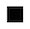
\includegraphics[width=0.8\textwidth]{square.jpg}}
    \caption{A 30x30 b/w square.}
  \end{center}
  \end{minipage}
  \hfill
   \begin{minipage}[b]{0.45\textwidth}
   \begin{center}
    \frame{
\includegraphics[width=0.8\textwidth]{circle_bw_lowres.jpg}}
    \caption{A 30x30 b/w circle.}
    \end{center}
  \end{minipage}
\end{figure}

The gradient magnitude histograms for square and circle:

\begin{figure}[H]
  \centering
  \begin{minipage}[b]{0.45\textwidth}
    \includegraphics[width=\textwidth]{square_gradnorm_histogram.png}
    \caption{Gradient magnitude of square.}
  \end{minipage}
  \hfill
    \begin{minipage}[b]{0.45\textwidth}
    \includegraphics[width=\textwidth]{circle_lowres_gradnorm_histogram.png}
    \caption{Gradient magnitude of circle.}
  \end{minipage}
\end{figure}

The pairwise gradient angle histograms for square and circle:

\begin{figure}[H]
  \centering
  \begin{minipage}[b]{0.45\textwidth}
    \includegraphics[width=\textwidth]{square_gradangle_histogram.png}
    \caption{Gradient angle of square.}
  \end{minipage}
  \hfill
    \begin{minipage}[b]{0.45\textwidth}
    \includegraphics[width=\textwidth]{circle_lowres_gradangle_histogram.png}
    \caption{Gradient angle of circle.}
  \end{minipage}
\end{figure}

More formally, gradient magnitude and pairwise gradient angle are defined as follows. 

Let $I(x,y)$ be the gray level of the pixel located at position $(x,y)$, then $g(x,y) = \nabla I(x,y)$ is the gradient and the square norm $|g|$ is the gradient magnitude. However, since this is working in a discrete setting, we need to specify how the gradient is discretized. I defined the discrete gradient as the average difference of two neighboring pixels \[g(x,y) = (g_x, g_y) = \left(\frac{I(x+1,y) - I(x-1,y)}{2},\frac{I(x,y+1)-I(x,y-1)}{2}\right)\]
On the edge of the image where there is only one side neighbor, then I just take that difference. And the feature is the square norm
\[F_1(x,y) = \|g(x,y)\|_2\]

The pairwise gradient angle is 
\[F_2(x_1,y_1,x_2,y_2) = \cos^{-1}\left(\frac{g_1^Tg_2}{|g_1||g_2|}\right),\] where
\[g_1 = g(x_1,y_1), g_2 = g(x_2,y_2)\]

One question to address is how to define the pairwise gradient angle when $|g_1| = 0$ or $|g_2| = 0$. I took the lazy approach to define it as 0, but this is artificial and there is likely a more clever way to define the gradient angle at zero gradients.

The empirical probability distribution $\hat P$ of the two global image statistics are collected from the entire image. For pairwise gradient angle, the angles are collected from all pairs of neighbors. When producing the histogram, I found that it practically works well to bin the gradient magnitude and angle into intervals of 0.05.

\section{Exponential Distribution}

With an exponential distribution model on the above two features, the probability of an image is given by
\[P(I; \Phi_1,\Phi_2) \propto \exp\left[\sum_{(x,y)}\Phi_1(F_1(x,y)) + \sum_{(x_1,y_1)\sim (x_2,y_2)}\Phi_2(F_2(x_1,y_1,x_2,y_2))\right]\]

To estimate $\Phi_1$ and $\Phi_2$ from the global image, the following estimation is adopted so that the predicted marginals of features match the empirical marginals in data.
\[\Phi_1(|g|) = \hat P(|g|)\]
\[\Phi_2(\theta) = \hat P(\theta)\]

Thus, our goal is to maximize the above expression of $P(I; \Phi_1,\Phi_2)$ in the hole.

\section{Simulated Annealing}

If we iterate over all possible hole configurations and brute force the maximization of $P(I; \Phi_1,\Phi_2)$, it would take too long since there are $|C|^N$ possible configurations where $C$ is the candidate set of grayscale color levels and $N$ is the size of the hole.

Instead of brute force, I used simulated annealing to approximate the best configuration to reduce computation time. The algorithm works as follows.

Define $V = \sum_{(x,y)}\Phi_1(F_1(x,y)) + \sum_{(x_1,y_1)\sim (x_2,y_2)}\Phi_2(F_2(x_1,y_1,x_2,y_2))$ to be the potential of a configuration. Let $h$ be the function $h(a) = \min(a,1)$.

\textbf{Step 0}: Initialize the hole with random grayscale colors sampled from a neighborhood.

\textbf{Step n+1}: 

- Choose a pixel in the hole and change it to a new random grayscale color sampled from the neighborhood.

- Choose a uniform random number $U$ from [0,1].

- Compute the new potential $V'$.

- Set the temperature to be $T = C / \log(n)$

- If $U < h(\exp[(V-V')/T])$, accept the new configuration and change that pixel. Otherwise, keep the old configuration.

\bigskip

In my implementation, I used an existing python simulated annealing package \textbf{simanneal}: 

https://github.com/perrygeo/simanneal

\section{Results}

The results are from simulated annealing with initial temperature 10000K, and the candidate grayscale color levels are sampled from a neighborhood around the hole with 3 times the size of the hole. 

In practice, I found it much better assign higher weights to $\Phi_1$ on the boundary of the hole, so that the inpainted filling blends better with the surroundings. Otherwise, it's very easy to obtain an undesired filling of all white or all black pixels (since zero gradient has the highest probability among gradient magnitudes). In the following results, the pixels on the boundary are weighted by the size of the hole, and inner pixels are weighted by 1.

The algorithm works well to fill holes with 10-20 pixels, but simulated annealing very soon becomes too slow as the hole grows larger. For the 7x7 hole in Figure 17-18, simulated annealing takes $>$ 10 minutes to run, and the result is not very desirable.

\begin{figure}[H]
  \centering
  \begin{minipage}[b]{0.45\textwidth}
  \begin{center}
    \frame{\includegraphics[width=0.8\textwidth]{figure_1-1.png}}
    \caption{A 30x30 arc with 1x10 hole.}
  \end{center}
  \end{minipage}
  \hfill
   \begin{minipage}[b]{0.45\textwidth}
   \begin{center}
    \frame{\includegraphics[width=0.8\textwidth]{figure_1-3.png}}
    \caption{Filled hole after 10000 iterations.}
    \end{center}
  \end{minipage}
\end{figure}

\begin{figure}[H]
  \centering
  \begin{minipage}[b]{0.45\textwidth}
  \begin{center}
    \frame{\includegraphics[width=0.8\textwidth]{figure_3-1.png}}
    \caption{A 30x30 circle with 3x3 hole.}
  \end{center}
  \end{minipage}
  \hfill
   \begin{minipage}[b]{0.45\textwidth}
   \begin{center}
    \frame{\includegraphics[width=0.8\textwidth]{figure_3-3.png}}
    \caption{Filled hole after 50000 iterations.}
    \end{center}
  \end{minipage}
\end{figure}

\begin{figure}[H]
  \centering
  \begin{minipage}[b]{0.45\textwidth}
  \begin{center}
    \frame{\includegraphics[width=0.8\textwidth]{figure_5-1.png}}
    \caption{A 30x30 square with 3x3 hole.}
  \end{center}
  \end{minipage}
  \hfill
   \begin{minipage}[b]{0.45\textwidth}
   \begin{center}
    \frame{\includegraphics[width=0.8\textwidth]{figure_5-3.png}}
    \caption{Filled hole after 50000 iterations.}
    \end{center}
  \end{minipage}
\end{figure}

\begin{figure}[H]
  \centering
  \begin{minipage}[b]{0.45\textwidth}
  \begin{center}
    \frame{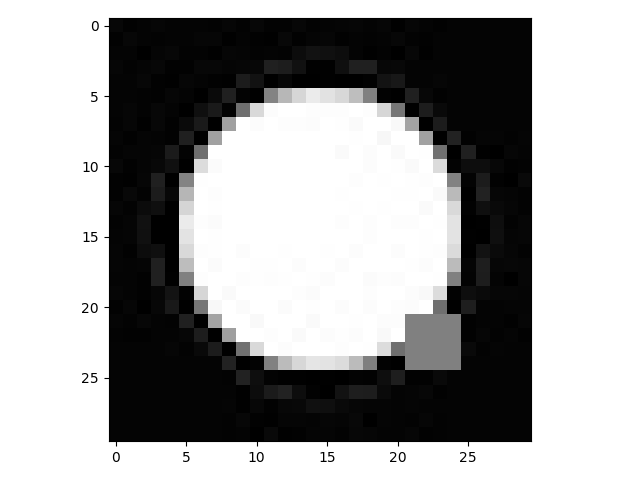
\includegraphics[width=0.8\textwidth]{figure_15-1.png}}
    \caption{A 30x30 circle with 4x4 hole.}
  \end{center}
  \end{minipage}
  \hfill
   \begin{minipage}[b]{0.45\textwidth}
   \begin{center}
    \frame{\includegraphics[width=0.8\textwidth]{figure_15-3.png}}
    \caption{Filled hole after 50000 iterations.}
    \end{center}
  \end{minipage}
\end{figure}

\begin{figure}[H]
  \centering
  \begin{minipage}[b]{0.45\textwidth}
  \begin{center}
    \frame{\includegraphics[width=0.8\textwidth]{figure_13-1.png}}
    \caption{A 30x30 circle with 7x7 hole.}
  \end{center}
  \end{minipage}
  \hfill
   \begin{minipage}[b]{0.45\textwidth}
   \begin{center}
    \frame{\includegraphics[width=0.8\textwidth]{figure_13-3.png}}
    \caption{Filled hole after 100000 iterations.}
    \end{center}
  \end{minipage}
\end{figure}

\section{Discussion}

When the hole is small and we have enough time in simulated annealing to find a close-to-optimal configuration, the inpainting looks reasonable to human eyes. However, simulated annealing is not fast enough to handle more than 20 pixels.

One observation we can make is that this choice of the exponential model can be seen as a Markov Random Field on the gradient field. There is a well-known optimization algorithm called \textbf{Max-product Belief Propagation} \cite{weiss2001optimality}. On simply connected graphs, this algorithm can find the optimal configuration, and on general graphs this algorithm approximates the optimal configuration \cite{weiss2001optimality}.

The next step of this project would be to implement max-product belief propagation and see if this inpainting model can handle larger holes.

It would also be interesting to experiment with other image statistics as features, such as log intensity, power spectrum, and wavelets \cite{pouli2011survey}. 

\bibliography{references} 
\bibliographystyle{ieeetr}

\appendix

\section*{Source Code}
\lstinputlisting[language=Python]{inpaint.py}

\end{document}
